\chapter{Evaluación experimental}
\label{chap:evaluacion_experimenal}
\lettrine{P}{ara} comprobar que os resultados obtidos correspóndense co plantexado neste capítulo probaremos o dispositivo BikeCam e a aplicación BikeView. Realizaremos probas en contornos controlados e probas no medio real o que esta dirixido e analizaramos se cumpre os requisitos legais.

\section{Consumo}

Comenzarase as probas medindo o consumo de amperios do sistema. Para elo colocarase un amperímetro usb entre unha fonte de alimentación e a conexión usb coa que alimentarase o sistema nestas probas. Repetiremos as probas con diferentes fontes de alimentación e distintos cables para descartar fallos e conseguir unha maior consistencia nos resultados. A continuación realizaranse as mesmas probas no dispositivo medindo o consumo alimentándoo coa batería.

Analizaranse os seguintes supostos para o dispositivo con un anel led e para o que conta a maiores coas dúas tiras led.
\begin{itemize}
    \item \textbf{Sistema en repouso: }
    O sistema esta aceso pero só se estean a executar as funcións do sistema operativo incluíndo o servidor ssh para o control remoto.
    \item \textbf{Servidor funcionando:}
    Executamos o servidor.
    \item \textbf{Cliente conectado:}
    Conectamos o dispositivo móbil o servidor.
    \item \textbf{Vídeo transmitindo:}
    Transmitimos vídeo en directo o dispositivo móbil.
    \item \textbf{Vídeo parado:}
    Paramos a transmisión de vídeo.
    \item \textbf{Desconexión do cliente:}
    Pechamos a aplicación no dispositivo móbil.
    \item \textbf{Luces intermitentes:}
    Iniciamos as luces intermitentes a máxima intensidade nunha das direccións, consumo varia no proceso, rexistremos o valor máximo.
    \item \textbf{Luces vermellas:}
    Acendemos as luces vermellas a intensidade máxima.
    \item \textbf{Luces vermellas e transmisión de vídeo:}
    Consumo coas luces vermellas a máxima intensidade e co vídeo transmitindo en directo.
\end{itemize}

\begin{figure}[tb]
  \centering
  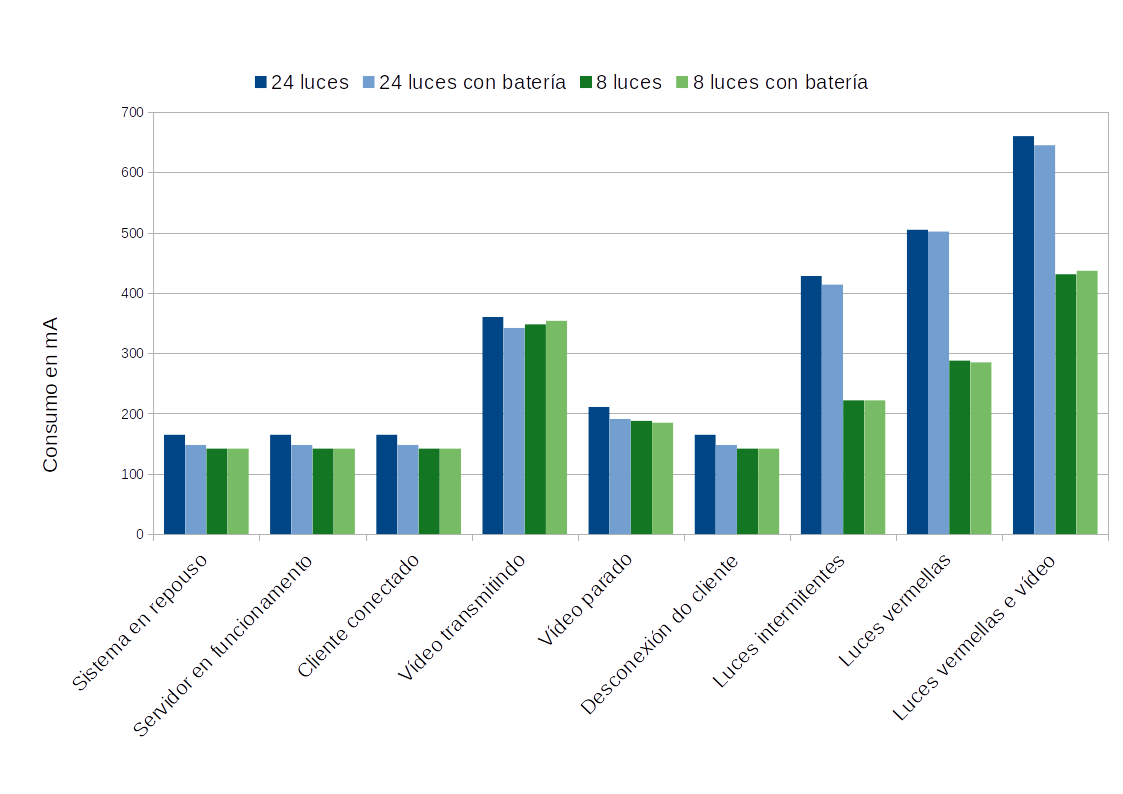
\includegraphics[scale=.5]{imaxes/grafica-amperaxe.png}
  \caption{Grafica do consumo en mA.}
  \label{fig:amperaxe}
\end{figure}
Como se pode observar na gráfica da figura~\ref{fig:amperaxe} o uso ou non de batería non afecta en gran medida ao consumo de amperios, pero ha de terse en conta que estas probas realizáronse coas batería coa carga completa. Se se compara a previsión de consumos feita coas medición obtidas
pódese ver que os valores no son moi diferentes sendo superior no caso do dispositivo de 8 luces, 437mA fronte aos 390mA previstos, e inferior no caso dispositivo con 24 luces, 660mA fronte aos 710mA previstos.
As fontes de alimentación utilizadas poden proporcionar un máximo de 3A e 2.1A respectivamente, tamén utilizáronse dous cables un de maior calidade e outro cunha calidade inferior. En ningún dos casos obtivéronse diferencias apreciables sendo a maior diferencia de 4mA. Na versión con batería necesitouse utilizar cableado a maiores para realizar as probas, o que pode que incrementara lixeiramente o consumo.

\section{Autonomía}

A seguinte proba a realizar será a de autonomía do dispositivo, para elo buscarase o consumo máximo acendendo as luces vermella a máxima intensidade o tempo que se transmite vídeo.


Comezaranse as probas co dispositivo dotado de batería interna, cando a voltaxe da batería esta entorno os 3.9V detectase un problema o sistema apagase, indicando batería baixa. O \emph{script} Python encargado de monitorizar o pin conectado o indicador de voltaxe baixo do Adafruit Powerboost detecta unha caída de voltaxe que confunde co franco de caída esperado cando o pin ponse a 0. O pin de baixo voltaxe do Adafruit Powerboost está conectado a voltaxe da batería cando a caga e superior a 3.2V e conectase a un valor de 0V cando baixa de este limite e debido a que cando batería esta a comezar a descargarse para poder proporcionar a amperaxe adecuada a súa voltaxe baixa a un ritmo rápido que confunde o \emph{script}. O podemos solucionar incluíndo unha segunda comprobación no \emph{script} despois de detectar o franco de caída comprobarase que o valor lido no pin é 0 antes de apagar a Raspberry.

A continuación detectase un segundo problema, despois de 15 min de funcionamento volvese a apagar por batería baixa e unha vez apagado a batería recuperase ata unha voltaxe de 3.6V. Esto debese a que o estar consumindo o máximo de amperios necesita baixar a súa voltaxe para poder seguir entregando estes amperios. Reducindo a intensidade dos leds conséguese a que o sistema non se apague pero a medida que a voltaxe vai baixando é necesario reducir a intensidade aínda máis.  Este problema pódese solucionar de dúas formas:
Utilizando un batería de maior capacidade xa que poderá seguir subministrando a amperaxe necesaria a menor voltaxe.
Utilizar unha batería cunha constante de descarga maior, isto é a capacidade máxima de amperios que pode subministrar en función da capacidade en amperios hora. A batería utilizada ten unha constante de descarga de 1C isto quere dicir que coa sua caga completa o fabricante garante que proporcione 1.6A funcionando con normalidade.
Ámbalas dúas solucións implican na practica unha batería de maior tamaño.

Procedemos a repetir a proba pero esta vez deshabitando o apagado automático, esperando a que o sistema se apague cando a voltaxe non sexa suficiente para manter a Raspberry acesa ou no peor caso cando o circuíto de protección que inclúe a batería a desconecte a unha voltaxe mínima habitualmente 2.5V. De non usar unha batería con circuíto de protección poderíamos danar a batería podendo incluso arder ou estoupar durante próximas cargas. Neste caso obtivéronse 35 minutos de funcionamento. A voltaxe medida na batería foi de 3.58V, un valor de voltaxe na que a batería aínda conserva parte da súa carga. Que o sistema se apague neste punto e conveniente para protexer a batería e prolongar a súa vida útil pero reduce o tempo de uso da batería, que poderíamos seguir usando sempre que non utilicemos o consumo máximo do dispositivo, por exemplo apagando a transmisión de vídeo. Comprobamos este suposto reconectando a batería e esta vez acendendo so as luces e a unha intensidade do 50\(\%\), obtivéronse neste caso 50 minutos máis de funcionamento ata que a batería se desconectou mediante o seu circuíto de protección, para que volva a activarse e necesario comezar a recargala, a voltaxe medida foi de 3.4V.


Para comprobar a viabilidade do apagado automático realizamos unha nova proba esta vez so co anel led acendido e a unha intensidade do 80\(\%\) e o vídeo transmitindo, neste suposto o sistema permanece acceso durante  min e a voltaxe da batería despois do apagado é de V.

Comezarase as probas para a versión do dispositivo sen luces intermitentes e alimentando por batería USB, faremos a proba cunha batería de  2600mA, despois de 3h e 30min e coa batería a unha voltaxe de 3.2V o vídeo deixa de funcionar pero os leds seguen a responder o pouco tempo o control dos leds tamén deixa de funcionar e a Raspberry se apaga pero as luces segue acesas se é esta a posición na que as deixamos,  o chegar a 4 horas de funcionamento das luces e unha voltaxe de 2.9V desconectamos o sistema, e o intentalo arrancar de novo a voltaxe no e suficiente para arrancar a Raspberry.

Durante esta proba tamén se monitorizou o consumo enerxético do dispositivo android executando BikeView, para esta proba utilizouse un dispositivo cunha pantalla de 6,3" unha batería de 4000mAh e co brillo de pantalla a metade de intensidade. O comezo da proba o dispositivo contaba co 100\(\%\) da batería o rematar a proba despois de 4h a batería restante era do 64\(\%\).

\section{Vídeo e lentes}
Como se pode observar nas capturas da figura figura as calidade de imaxe e considerablemente maior cando se utiliza a versión 2 da cámara, esta diferenza é aínda máis notable cando as condicións de iluminación son desfavorables.

Na figura figura podemos observar captura de imaxe realizadas con diferentes lentes. Tódalas capturas son realizadas coa versión 2 da cámara para poder comparalas nas mesmas condicións. Probamos 3 lentes de amplitude distintas que situamos sobre a cámara figura figura, e outras 3 que se colocan na cámara con soporte para lentes figura figura.

Para medir a latencia gardaremos a captura de vídeo do dispositivo BikeCam gravando un cronómetro o tempo que grava a pantalla do dispositivo BikeView. Analizando posteriormente o vídeo calcúlase a latencia parando o vídeo e restando o valor do cronometro visualizado da pantalla menos o valor real do cronómetro como se aprecia na figura~\ref{fig:latencia}. Repetindo o procedemento en varios puntos do vídeo observamos unha latencia constante de entorno a 320ms para as probas realizadas coa versión un da cámara e 295ms para os probas coa versión 2.
\begin{figure}[tbp]
  \centering
  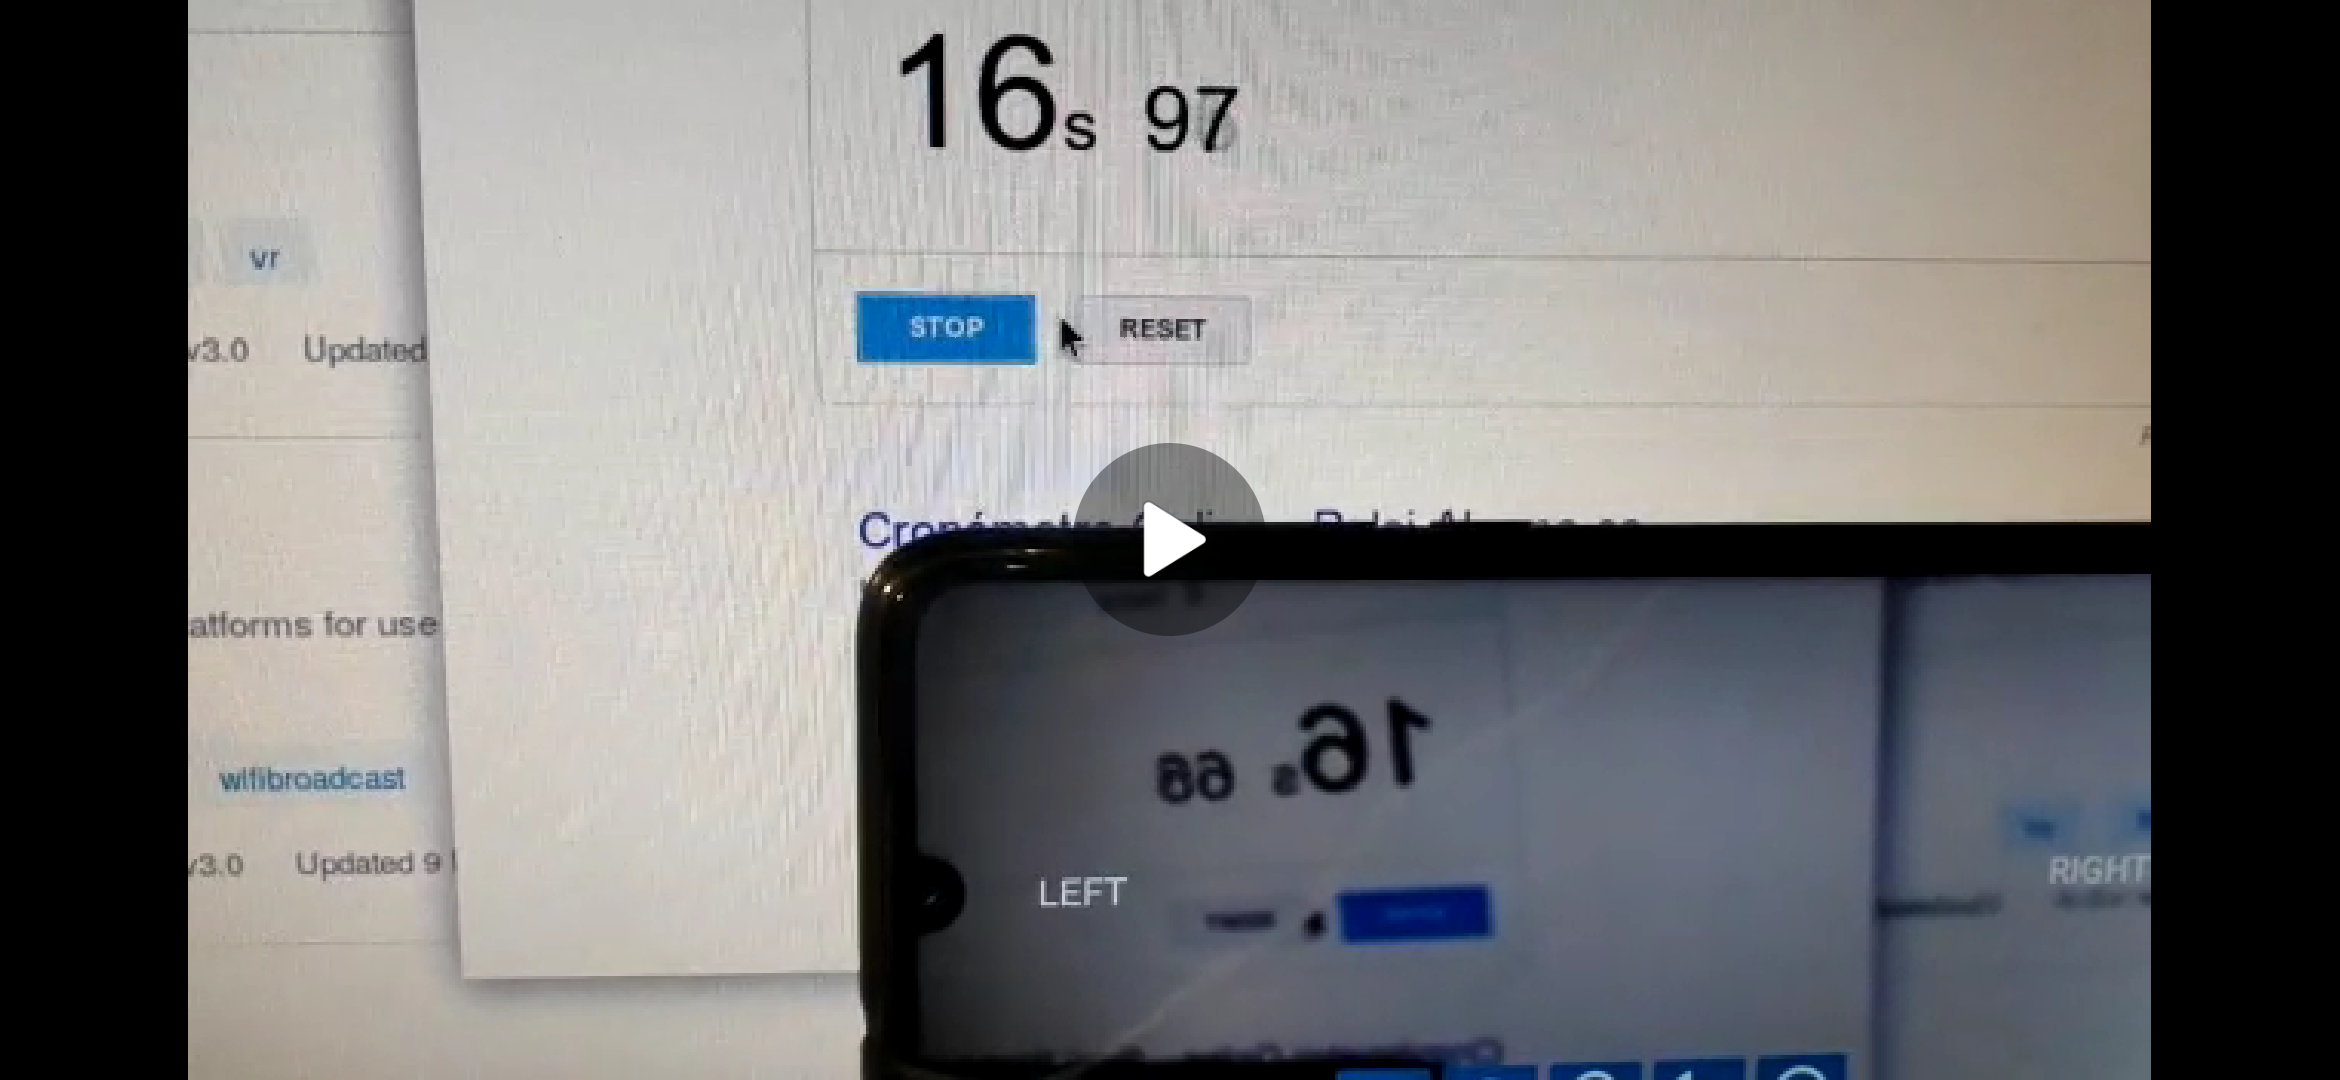
\includegraphics[scale=0.1]{imaxes/latencia.png}
  \caption{Medición empírica da latencia, pode observarse unha diferenza de 0,31 segundos.}
  \label{fig:latencia}
\end{figure}
Cabe destacar que na proba de autonomía realizada no dispositivo BikeCam con 24 leds cando este se encontraba a un nivel baixo de batería e un consumo máximo, \emph{streaming} de vídeo e máxima intensidade de luces, apreciouse nalgún momento subidas repentinas de latencia e defecto na imaxe seguramente devidos a faios de codificación.

\section{Visibilidade}
Para comprobar a visibilidade das luces procedeuse a observar o seu funcionamento a diferentes intensidades e distancias repetindo as probas de día e de noite. Sendo as luces amarelas máis brillantes e o padrón de movemento máis visible decidiuse facer as probas só nas luces vermellas e sen palpadeo para ilustra o caso menos visible.

As distancias elixidas para a proba foron 50, 100 e 150 metros e as intensidades elixidas 20, 40, 80 e 100 por cento.
Nas visualizacións realizadas de día a luz vermella era distinguible en todas as distancias e non se apreciaron diferenzas entres as distintas intensidades, isto pode deberse a que as intensidades utilizadas seguen unha escala lineal mentres que a percepción visual do ser humano se rexe por unha escala logarítmica, figura~\ref{fig:percepcion_luminica}, podería cambiarse a escala da regulación de intensidade por unha logarítmica para conseguir unha representación máis realista.
\begin{figure}[tbp]
  \centering
  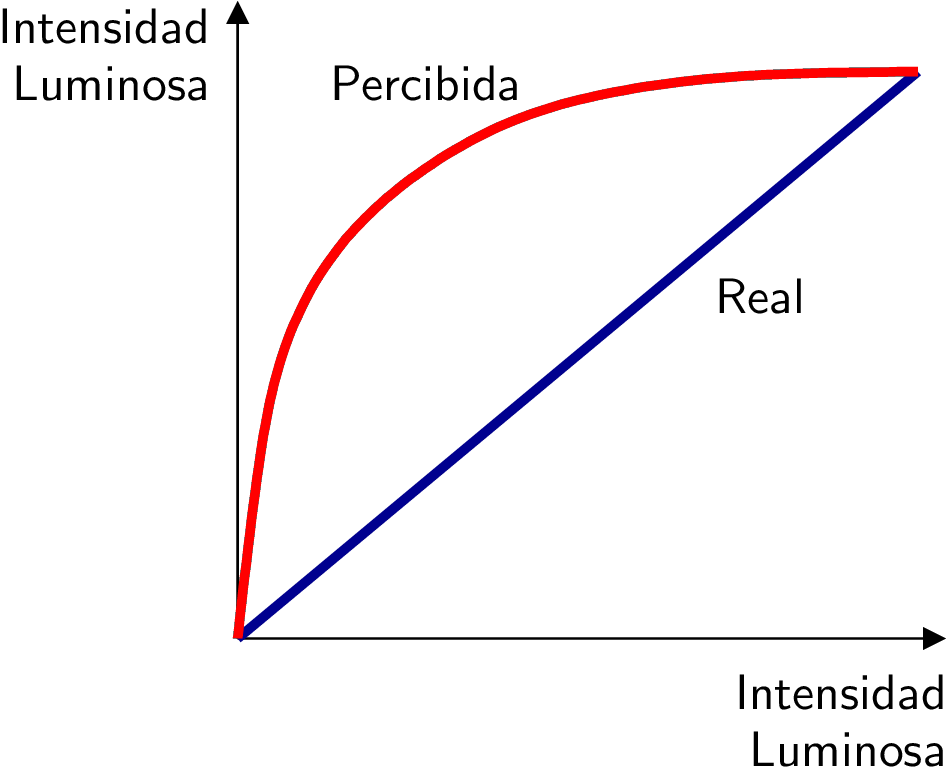
\includegraphics[scale=0.2]{imaxes/percepcion-luminica.png}
  \caption{Perecepción subxectiva de estímulos lumínicos segundo a lei de Weber-Fechner~\cite{PercepionVisual}.}
  \label{fig:percepcion_luminica}
\end{figure}

Nas visualizacións realizadas de noite as luces se percibía mellor que de día e neste caso si se podía distinguir as intensidades máis baixas das máis altas. Na figura~\ref{fig:fotos_distancia} móstranse unhas fotos da luz a intensidade máxima a 150m de día e de noite. Na figura~\ref{fig:foto_coche} mostrase a luz a 80\(\%\) a 150m comparada coas luces de freada dun coche a mesma distancia.

\begin{figure}[tbp]
  \centering
  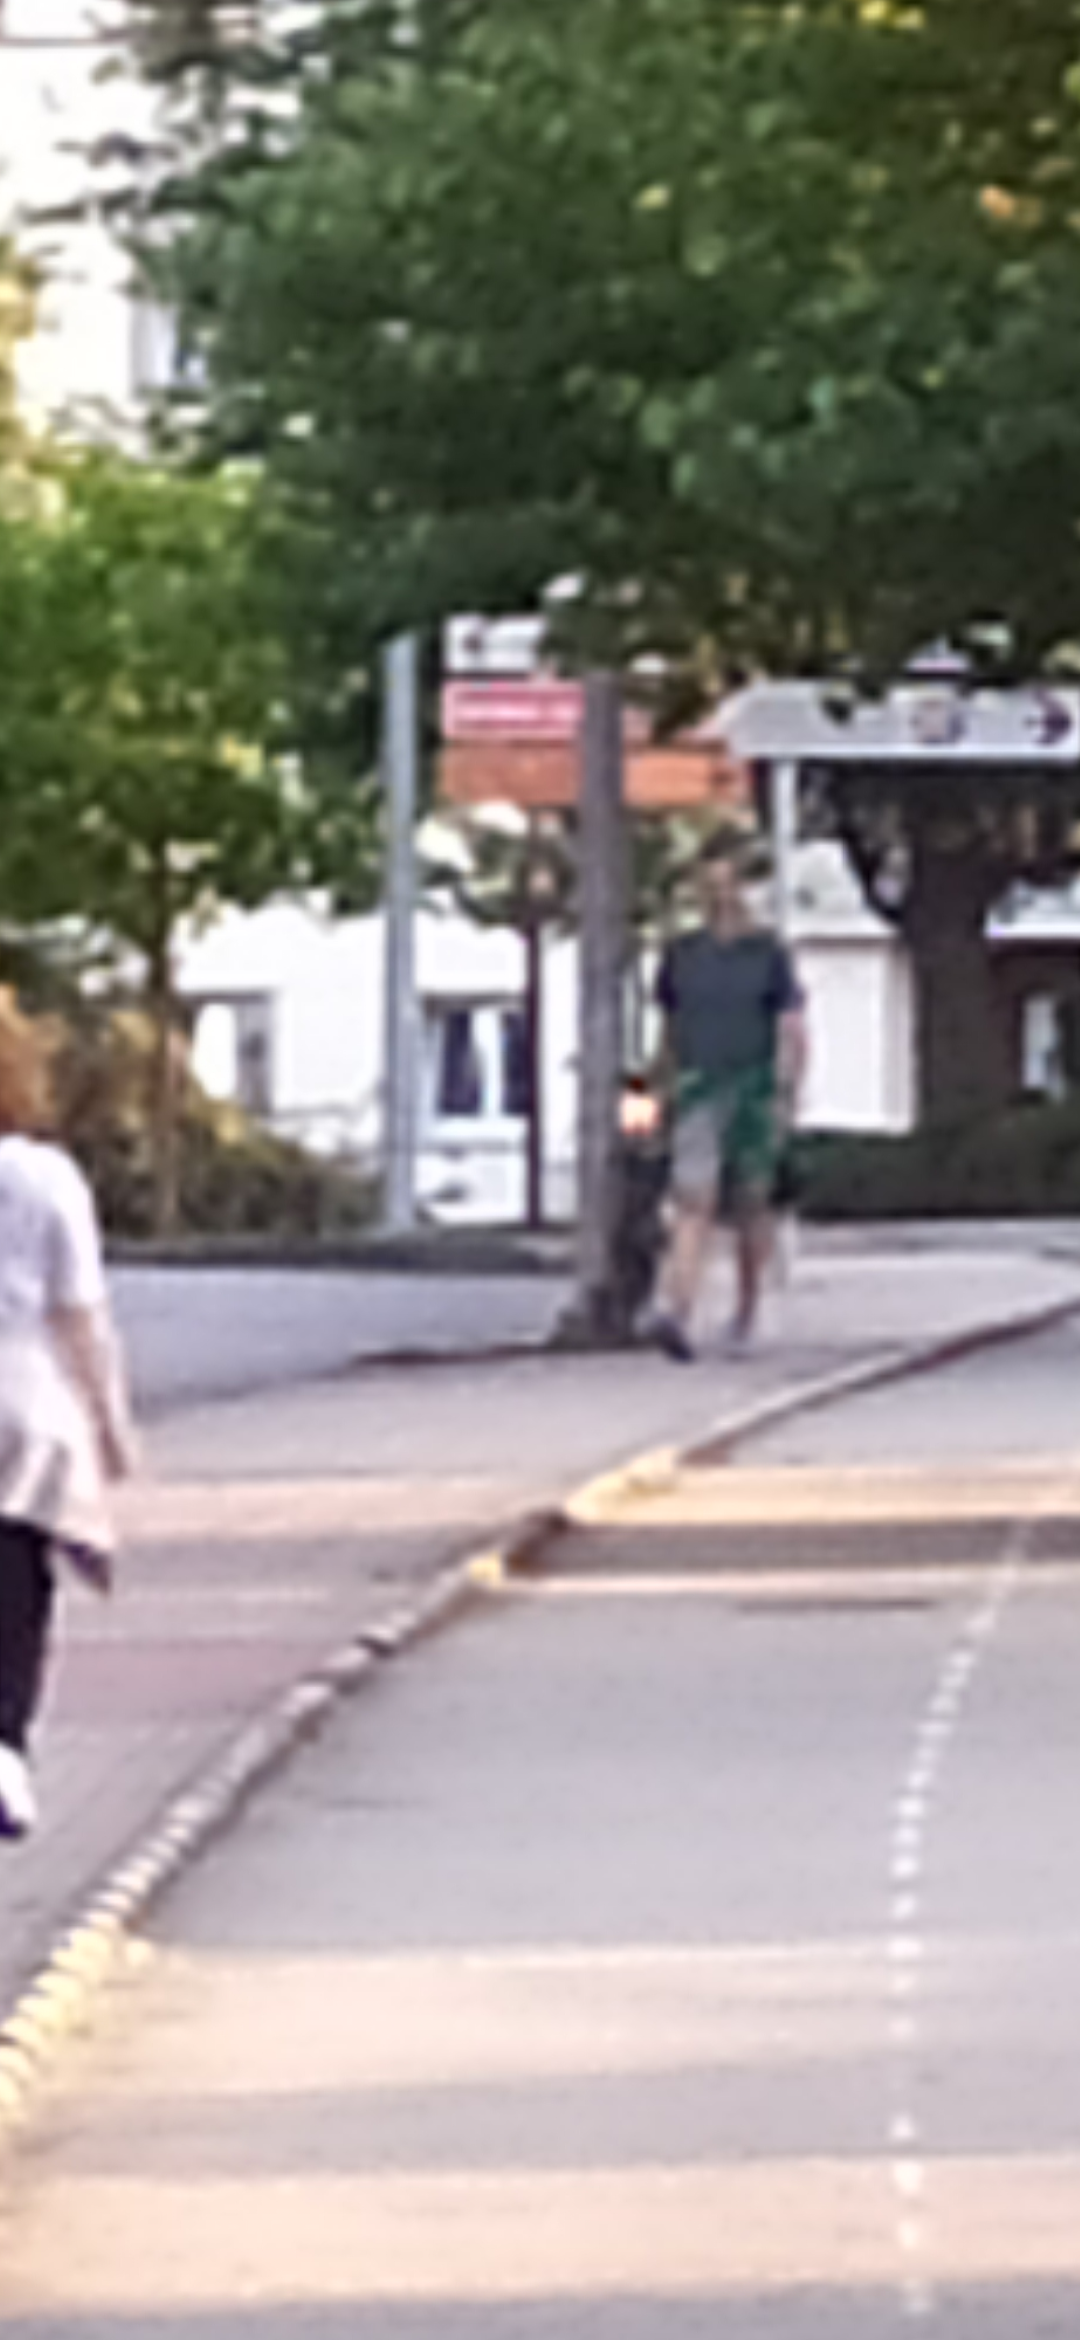
\includegraphics[scale=0.1]{imaxes/foto-dia.png}
  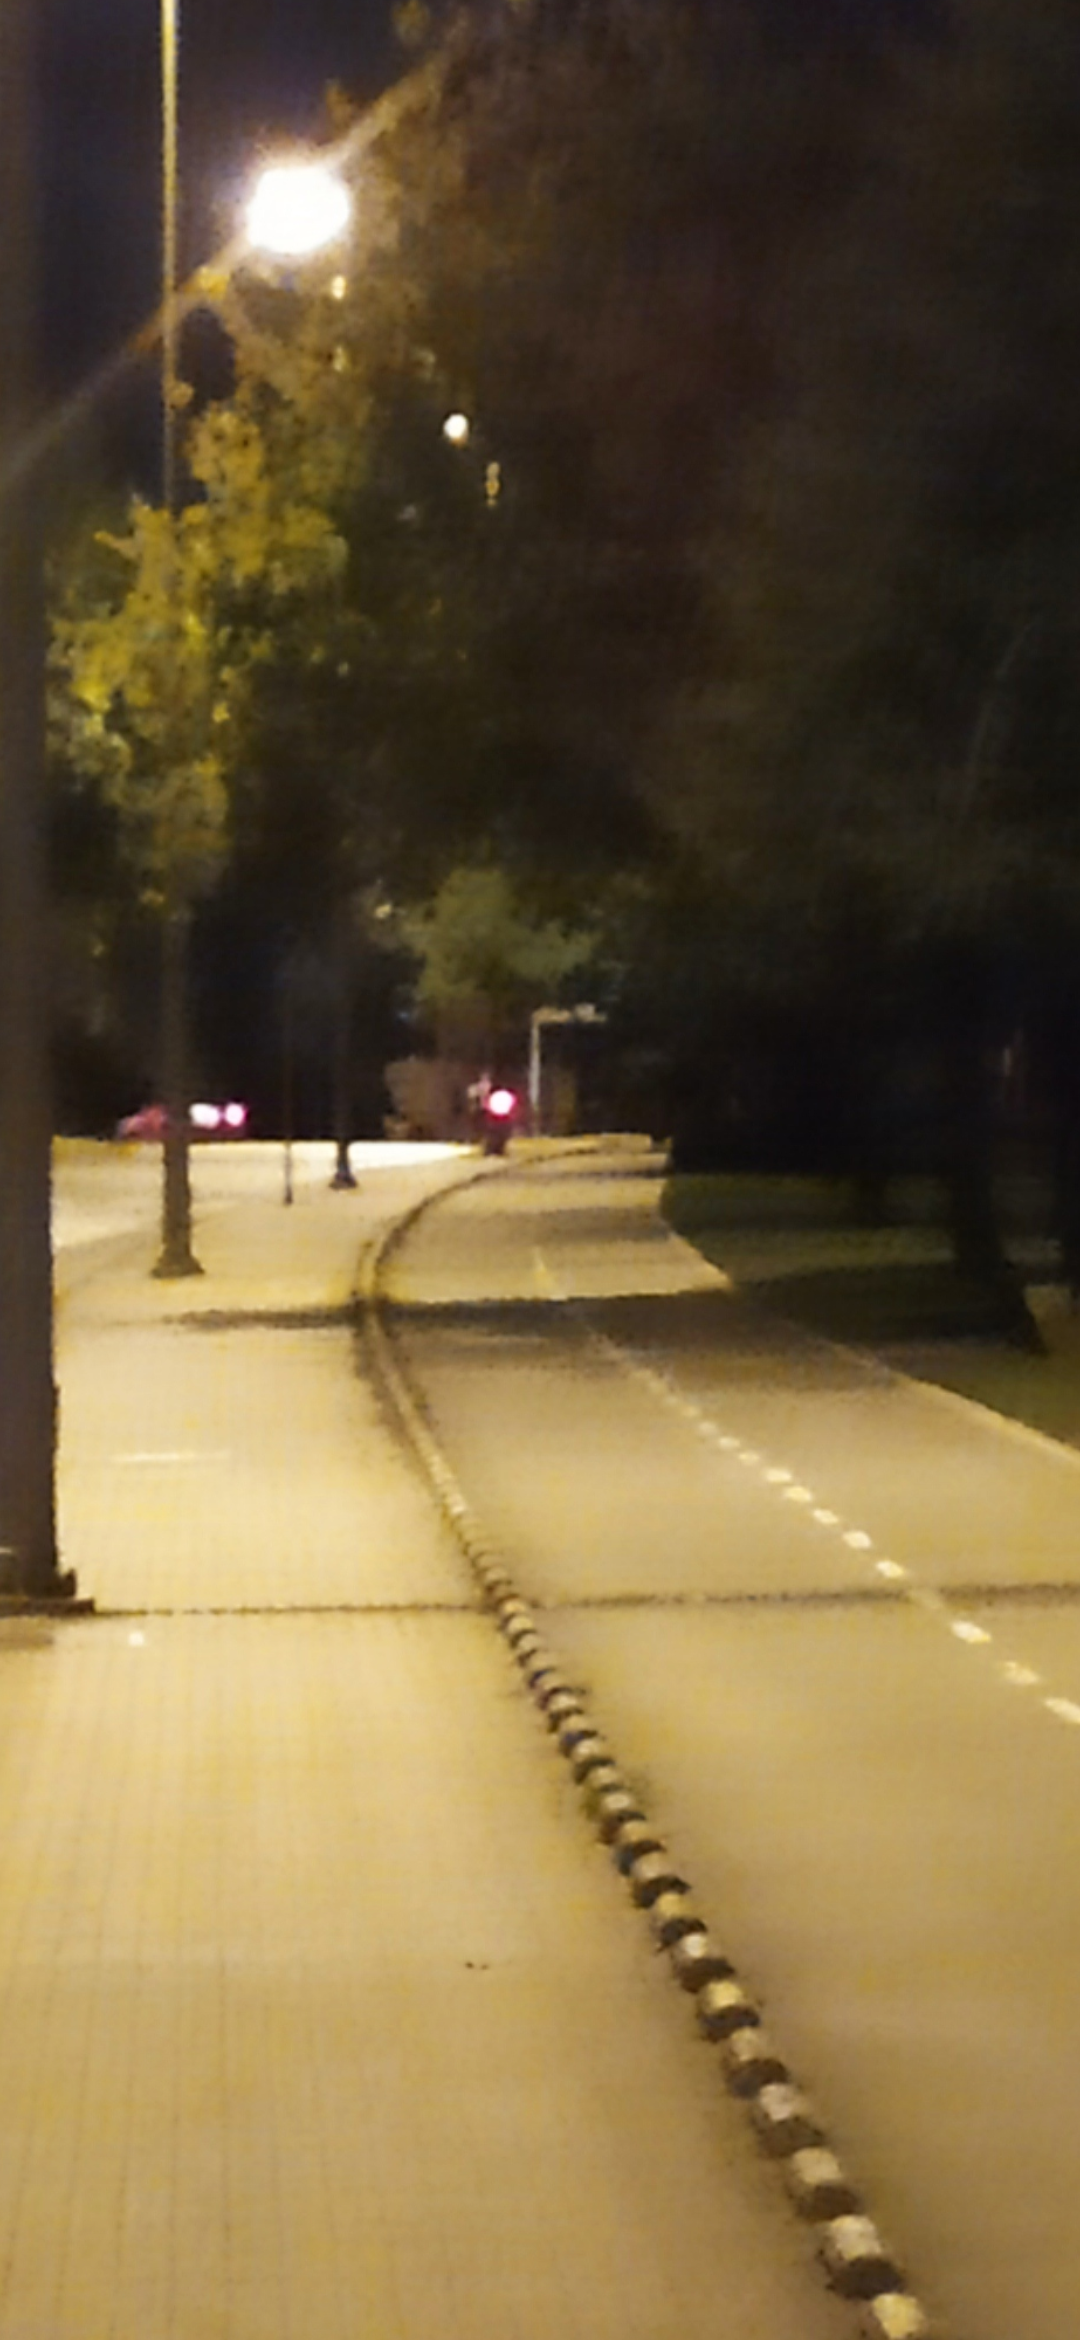
\includegraphics[scale=0.1]{imaxes/foto-noite.png}
  \caption{Fotos (recortadas) da luz vermella a 150m. A esquerda de día a dereita de noite.}
  \label{fig:fotos_distancia}
\end{figure}

\begin{figure}[tbp]
  \centering
  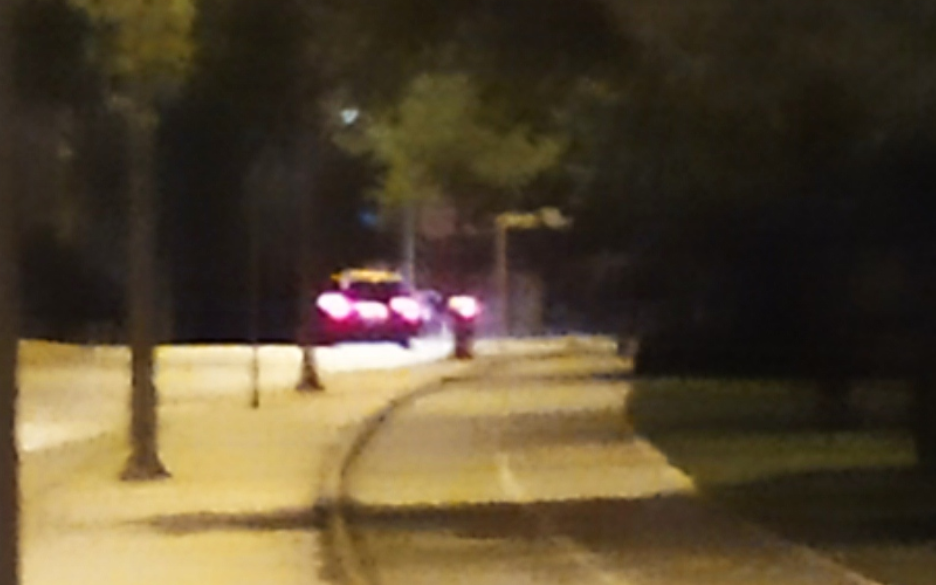
\includegraphics[scale=0.8]{imaxes/foto-coche.png}
  \caption{Comparación das luces vermellas xunto as luces de freada dun coche a 150m.}
  \label{fig:foto_coche}
\end{figure}

\section{Modo noite e freo automático}
Para comprobar o correcto funcionamento destes dous modos situouse o telefono no guiador da bicicleta e se realizaron as seguintes probas.
Comprobouse que no modo noite a luz vermella se acendía automaticamente ao entra nun túnel e se apagaba o saír de este, tamén se comprobou que se acendía correctamente ao solpor. Se ben o valor de luminosidade foi o adecuado podería ser conveniente que o usuario puidera controlar este limiar de luminosidade mínima.

As probas de deceleración realizáronse freando coa bicicleta en vías con diferente inclinación e co dispositivo Android tanto en posición horizontal como posición vertical. As luces acendéronse correctamente cando a bicecleta realia unha redución de velociade. De igual forma que co sensor de luminosidade seria conveniente que o usuario puidera establece o mínimo limiar de forza de deceleración a que quere que se acenda as luces.


\section{Lexislación}
A Lexislación que regula o uso de luces e cámaras varía amplamente segundo o país, analizaremos a legalidade do dispositivo segundo a lexislación española.

\subsubsection{Luces}
O uso de luces en bicicleta e obrigatorio en España cando as condicións lúminicas son insuficientes, na Instrución 18/S-146 da Dirección Xeneral de Tráfico con respecto a legalidade de luces parpadeantes, detalla os requisitos lumínicos aplicables as bicicletas recollidos nas diferentes lexislacións~\cite{Instruccion18S146}:
\begin{itemize}
  \item Artigo  98.1  do  Regulmento  Xeneral  de Circulación, aprobado por Real Decreto 1428/2003, de 21 de novembro.\\
  "Todos los vehículos que circulen entre el ocaso y la salida del sol o a cualquier hora del día en los túneles, pasos inferiores y tramos de vía afectados por la señal “túnel” (S-5) deben llevar encendido el   alumbrado   que   corresponda   de   acuerdo   con   los   que   se determina en esta sección".
  \item  Regulamento Xeneral de Vehículos, aprobado por Real Decreto 2822/1998, de 23 decembro\\
  "En el artículo 22.4 se indica que las bicicletas, para circular de noche, por tramos   de   vías   señalizados   con   la   señal   de   “túnel”   o   cuando   existan condiciones  meteorológicas  o  ambientales  que  disminuyan  sensiblemente  la visibilidad,  deberán  disponer  de  los  siguientes  dispositivos: luz  de  posición delantera   y   trasera,   catadióptrico   trasero,   y   podrán   disponer   de catadióptricos en los radios de las ruedas y en los pedales".
  \item Real Decreto 339/2014, de 9 de mayo, que establece os requisitos para a comercialización e posta en servizo das bicicletas e outros ciclos e as súas partes e pezas,establece no Anexo V o rango de intensidade lumínica nos faros das bicicletas (ver figura~\ref{fig:lexislacion_luminica}).

  \begin{figure}[tbp]
    \centering
    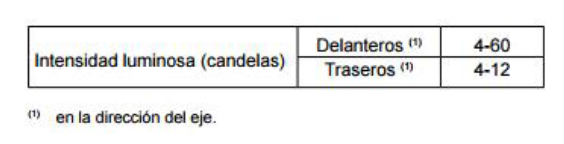
\includegraphics[scale=0.6]{imaxes/lexislacion-luminica.png}
    \caption{Rango de intensidade lumínica nos faros das biciletas en España~\cite{Instruccion18S146}.}
    \label{fig:lexislacion_luminica}
  \end{figure}
\end{itemize}

A instrución conclúe que o uso de luces parpadeantes é legal sempre que as luces no produzan cegamento o resto de usuarios da vía e se adecúen a normativa citada.
Para saber se as luces cumpren estes requisitos lumínicos tense que calcular as candelas que emiten. Os fabricantes de tiras leds raramente indican esta información e se o fan é en formato de lúmenes que para converter a candelas e necesario saber o ángulo de emisión, dato que tampouco facilitan, e non tódolos leds co mesmo formato compórtanse da mesma maneira. Na ficha técnica duns leds WS2812B, coma os utilizados neste proxecto, do fabricante Worldsemi~\cite{WS2812BDatasheet} na táboa~\ref{tab:intensidade_leds} especifican as milicandelas dos seus leds, tendo unha intensidade lumínica máxima combinada de entre 1850 e 2500 milicandelas.

O dispositivo desenvolto so utiliza dúas cores a vermella cun valor \emph{RGB} (255,0,0) e a amarela cun valor \emph{RGB}  (255,170,0). Polo tanto para a luz vermella solo utilizamos este led cunha intensidade máxima indicada na táboa deste fabricante de entre 550 en 700 milicandelas. Para a luz amarela o led vermello funciona a intensidade máxima e o verde cun valor de 177 dun máximo de 255, supoñendo unha transmisión lineal destes valores a intensidade en candelas, obteríase un valor do 69.4\(\%\) que sobre os datos do fabricante para o led verde resulta entre 763 e 961 milicandelas, sumados os valores do led vermello o resultado é un máximo de entre 1313 e 1661 milicandelas.

Para a luz vermella, no dispositivo de 8 luces isto serán entre 4.4 e 5.6 candelas, dentro do rango legal de entre 4 e 12 candelas, no caso do dispositivo de 24 luces o intensidade máxima será de entre 13.2 e 16.8 candelas en principio superior o limite legal non obstante este requirimento de intensidade é na dirección do eixo e as 16 luces extras utilizadas neste dispositivo están colocadas nun ángulo duns 55 graos polo que a intensidade na dirección será inferior, non e posible calcular este valor sen coñecer o ángulo de emisión de luz de estes leds.
Para a luz amarela entre 10.5 e 13.2 candelas, podendo ser neste caso superior o limite legal, no dispositivo de 24 luces o valor máximo será de entre 31.5 e 39.8 candelas aínda que de igual forma que as vermellas o valor na dirección do eixo será menor.

Como se pode observar en tódolos casos, a priori, as luces acadan o limite legal pero nalgúns o sobrepasan, para adaptar o comportamento das luces a lexislación bastará con limitar o valor da intensidade máxima. Para poder obter este valor será necesario realizar probas empíricas para medir as candelas emitidas polo dispositivo.

Cabe destacar que o uso de indicadores de xiro non está recollido na lexislación española polo que seu uso podería ser sancionable si se considera que pode ser contraproducente cegando a visión doutros ocupantes da vía. O seu uso non eximirá a necesidade de indicar as manobras co brazo como require a lei.
\begin{table}[tb]
  \caption{Características dos leds WS2812B de Worldsemi}
    \label{tab:intensidade_leds}
    \begin{center}
        \begin{tabular}{|l|l|l|l|l|}
            \hline
             Cor a emitir & Modelo & Lonxitude de onda (nm) & Intensidade lumínica (mcd)&Voltaxe(V)\\ \hline
             Vermello & 13CBAUP & 620-630 & 550-700 & 1.8-2.2\\ \hline
             Verde & 13CBAUP & 620-630 & 1100-1400 & 3.0-3.2\\ \hline
             Azul & 10R1MUX & 465-475 & 200-400 & 3.0-3.4\\ \hline
        \end{tabular}
    \end{center}
\end{table}

\subsection{Cámaras}

Como o dispositivo non almacena as imaxes capturadas nin as comparte con terceiros non se esta a vulnerar ningunha lexislación. De incorporar a opción de gravar a vía poderíase incorrer nun delito nalgúns casos, xa que non existe unha regulación concreta sobre este tipo de cámaras.
 Non será legal gravar a vía publica se se realiza de forma continuada e co vehículo parado xa que se pode considerar vídeo vixilancia ilegal, pero poderase capturar imaxes en movemento sempre que a utilización de estas se restrinxa o uso privado xa que a compartición de imaxes de persoas e das matriculas dos vehículos na vía pública vulnera a Ley Orgánica de Protección de Datos de Carácter Personal (LOPD)~\cite{BOEEsDocumento} sempre que non se conte co consentimento destas persoas. En caso de accidente as imaxes poderían utilizarse nun xuízo ou nunha reclamación o seguro só con autorización xudicial.
